\documentclass[10pt]{beamer}

\usetheme{metropolis}
\usepackage{appendixnumberbeamer}

% \usepackage[font=small]{caption}
\usepackage{booktabs}
\usepackage[scale=2]{ccicons}
\usepackage{natbib}
% \usepackage[font=small]{caption}

\usepackage{pgfplots}
\usepgfplotslibrary{dateplot}

\usepackage{xspace}
\newcommand{\themename}{\textbf{\textsc{metropolis}}\xspace}

\graphicspath{ {images/} }


\title{The Role Of L-Lactate In Sleep And Torpor Regulation}
\subtitle{Graduate Coursework}
\date{\today}
\author{\textbf{Student:} Minkow W. A. \\ \textbf{Scientific Adviser:} Gelfand M. S. \\ \textbf{Consultant:} Panchin Y. V.}
\institute{National Research University – Higher School of Economics \\ Faculty of Computer Sciences}
% \titlegraphic{\hfill\includegraphics[height=1.5cm]{logo.pdf}}

\begin{document}







\maketitle

\begin{frame}{Table of contents}
  \setbeamertemplate{section in toc}[sections numbered]
  \tableofcontents[hideallsubsections]
\end{frame}





\section{Introduction}

\begin{frame}[fragile]{Research Description}

\begin{itemize}
  \item Mammals exhibit a great diversity of sleeping patterns
  \item Various adapting thermoregulating mechanisms
  \item Longitude polygraphic study of naked mole-rats and Mongolian hamsters
  \item L-lactate as agonist and D-lactate antagonist injection in rats
  \item Phylogenetic tree of lactate receptors 
\end{itemize}

\end{frame}


\begin{frame}[fragile]{Allocricetulus curtatus}

\begin{figure}[H]
\centering
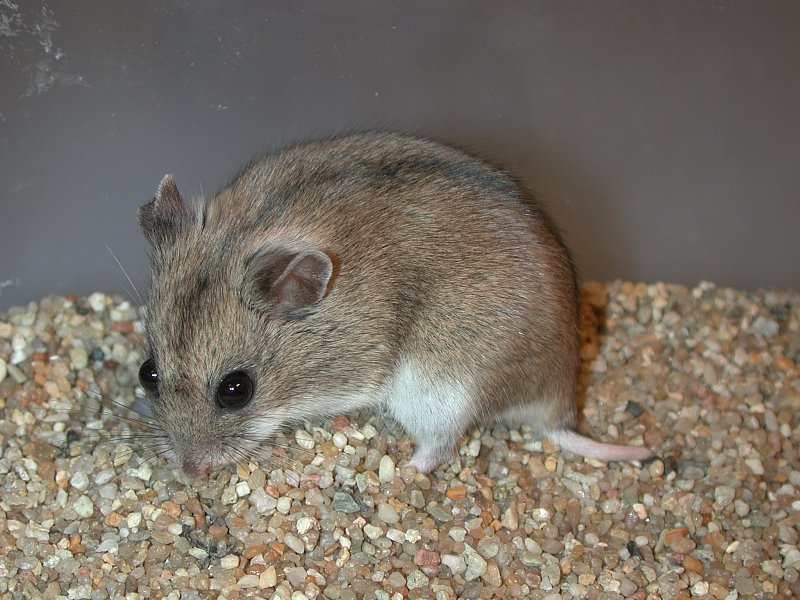
\includegraphics[width=0.7\linewidth]{curtatus.jpg}
\caption{Mongolian hamster (Allocricetulus curtatus) is a rodent species. Belongs to the family Cricetidae. Small, but larger than the mouse. The color is very light. The coat is flat. It is found in the south of Tuva, in China and in Mongolia.}\label{fig:curtatus}
\end{figure}

\end{frame}


\begin{frame}[fragile]{Heterocephalus glaber}

\begin{figure}[H]
\centering
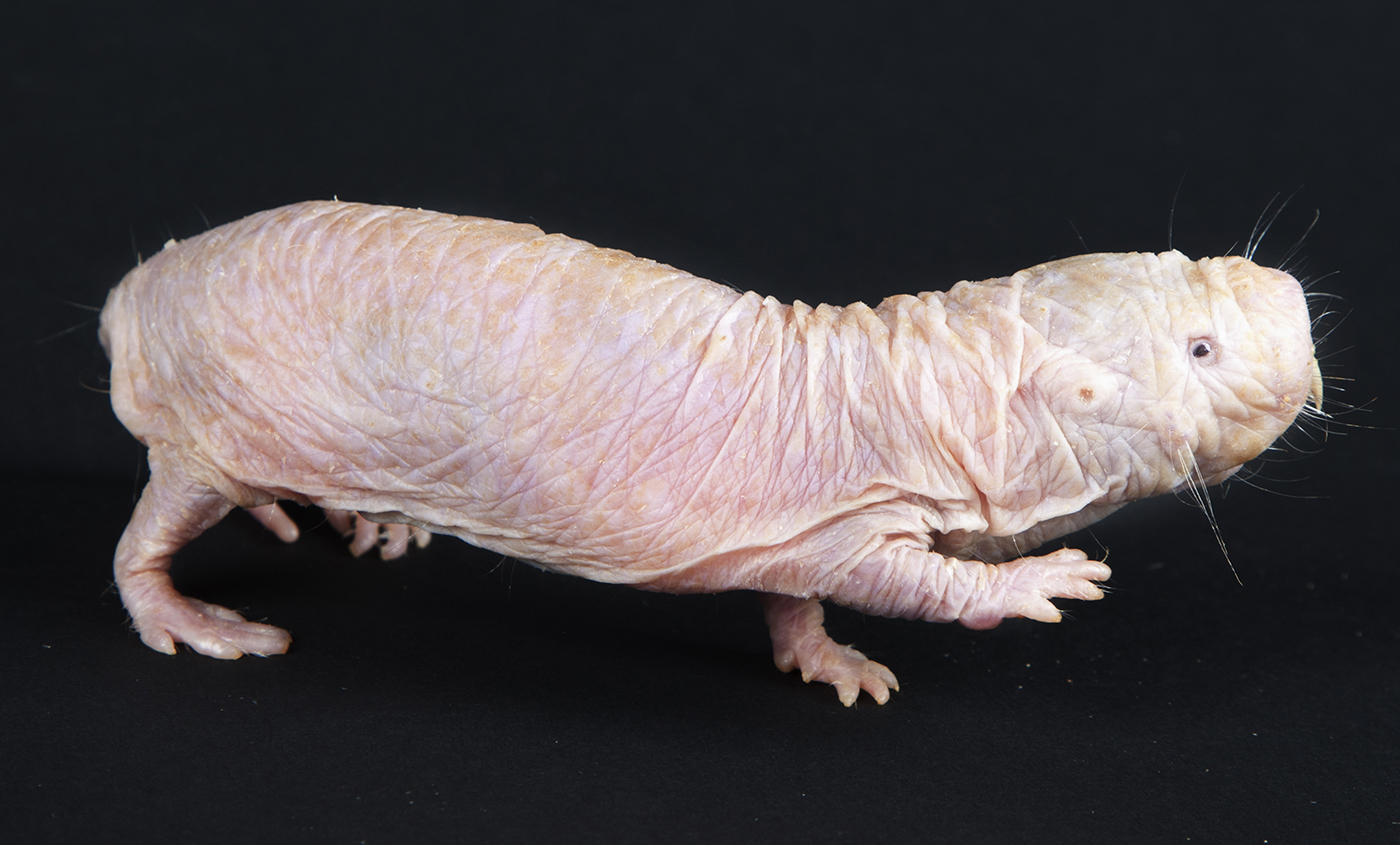
\includegraphics[width=0.7\linewidth]{nakedmolerat.jpg}
\caption{Naked mole-rat (\textit{Heterocephalus glaber}), or sand puppy, are burrowing rodents of the family Bathyergidae. The species is distinguished by unique features for mammals: a complex social organization of the colony, cold blood, insensitivity to some forms of pain. Appearance indicates the adaptation to the underground lifestyle. Found in East Africa, especially in Ethiopia.}\label{fig:nakedmolerat}
\end{figure}

\end{frame}


\begin{frame}[fragile]{L-lactate receptors}
\begin{figure}[H]
\centering
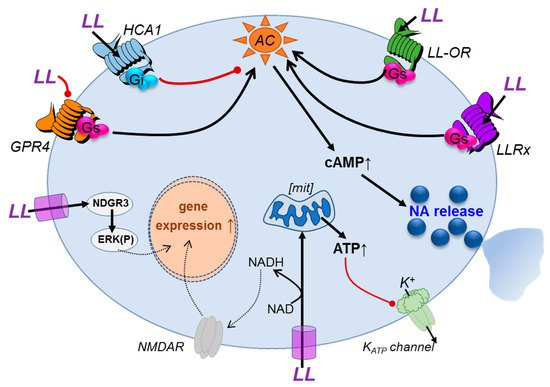
\includegraphics[width=0.7\linewidth]{lactate_receptors.jpg}
\caption{"Summary of potential l-lactate (LL)-mediated signalling actions in neurones. l-lactate which is transported into the cell can be metabolised and/or influence gene expression, e.g., via NMDA receptor modulation or ERK pathway activation." \citep{Mosienko2018}}\label{fig:lactate_receptors}
\end{figure}
\end{frame}

\section{The Hamster Experiment}

\begin{frame}[fragile]{The First Hamster}
\begin{figure}[H]
\centering
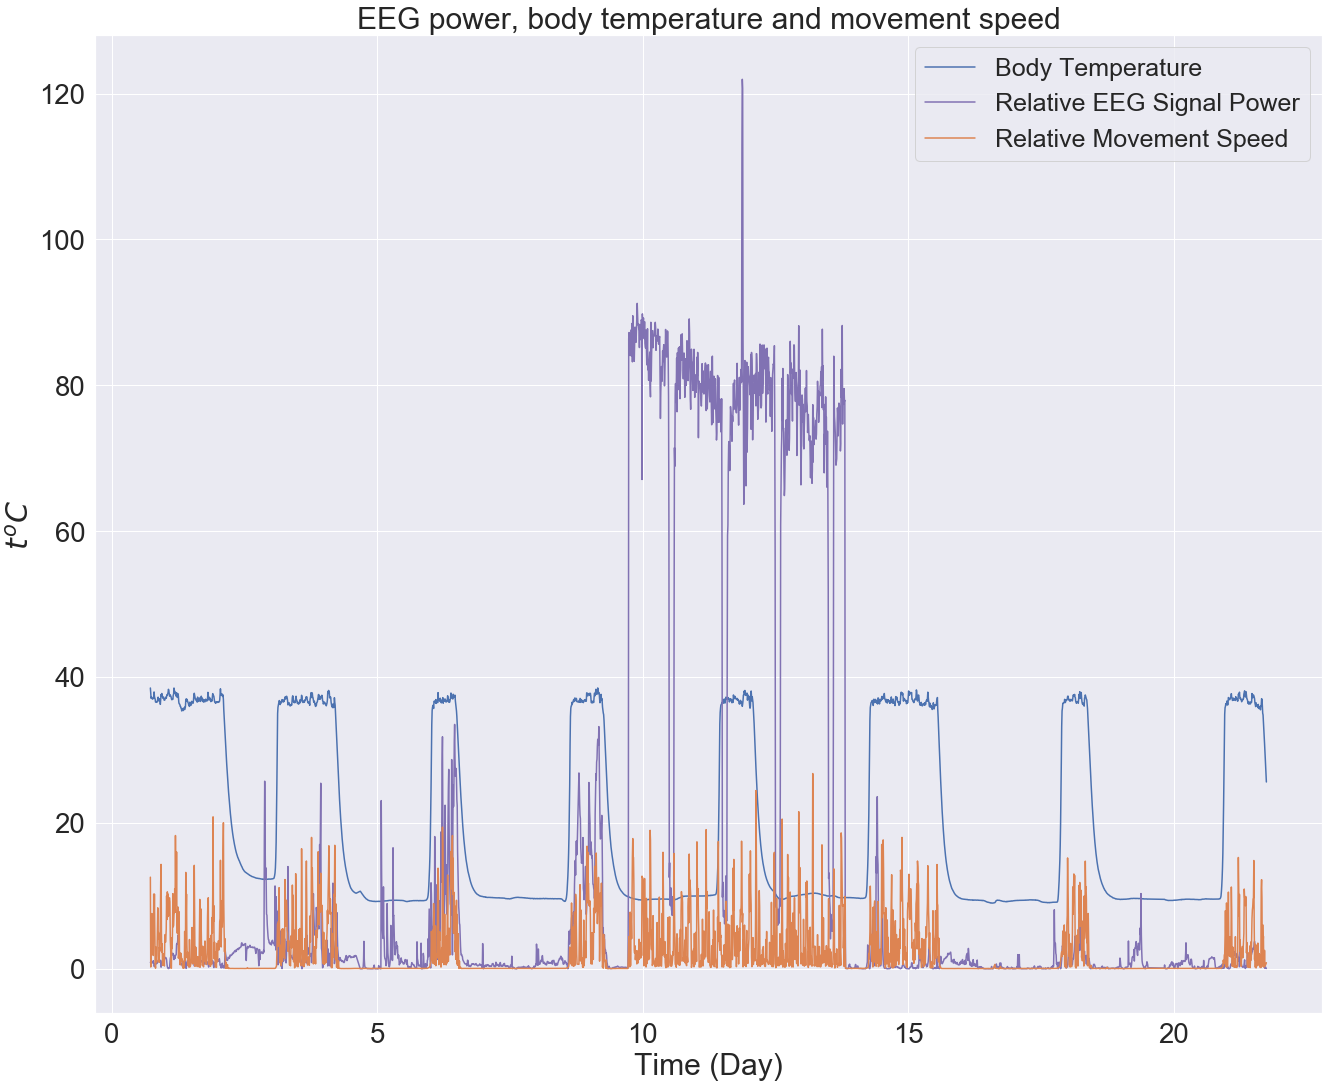
\includegraphics[width=0.7\linewidth]{exp1_1.png}
\caption{The graph shows the body temperature of a hamster as a function of time, scaled movement speed and scaled values of EEG power. The part with a large artifact is not deleted. All measurements are presented.}\label{fig:lactate_receptors}
\end{figure}
\end{frame}

\begin{frame}[fragile]{The First Hamster}
\begin{figure}[H]
\centering
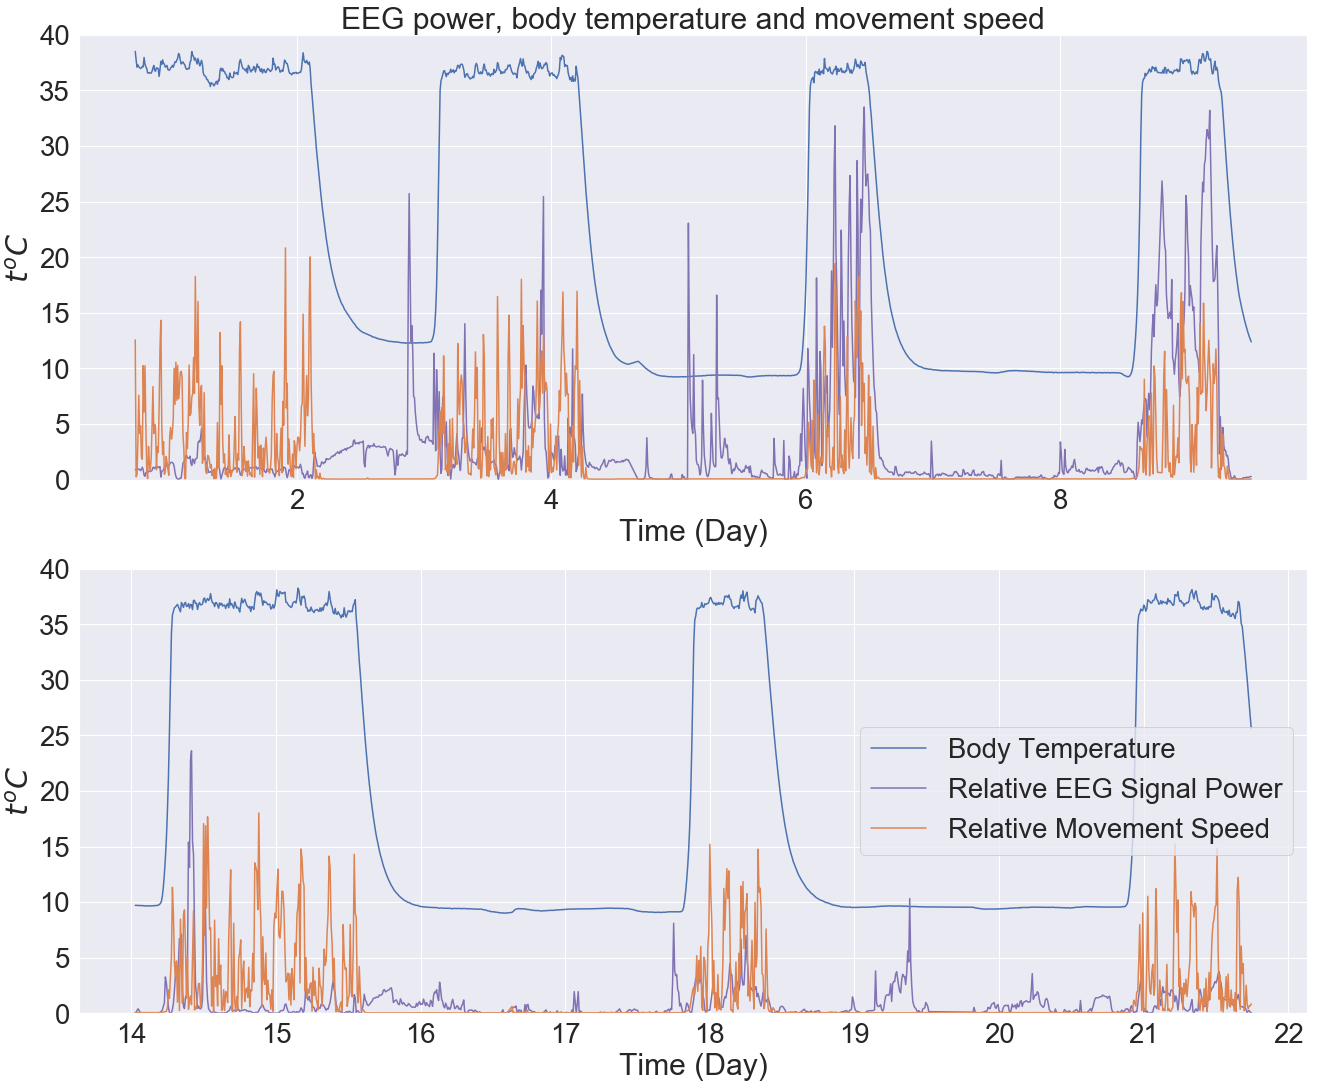
\includegraphics[width=0.7\linewidth]{exp1_2.png}
\caption{The graph shows the body temperature of a hamster as a function of time, scaled movement speed and scaled values of EEG power. The part with a large artifact, located in the middle, is removed. The schedule is divided into two parts for convenience.}\label{fig:lactate_receptors}
\end{figure}
\end{frame}


\begin{frame}[fragile]{The First Hamster}
\begin{figure}[H]
\centering
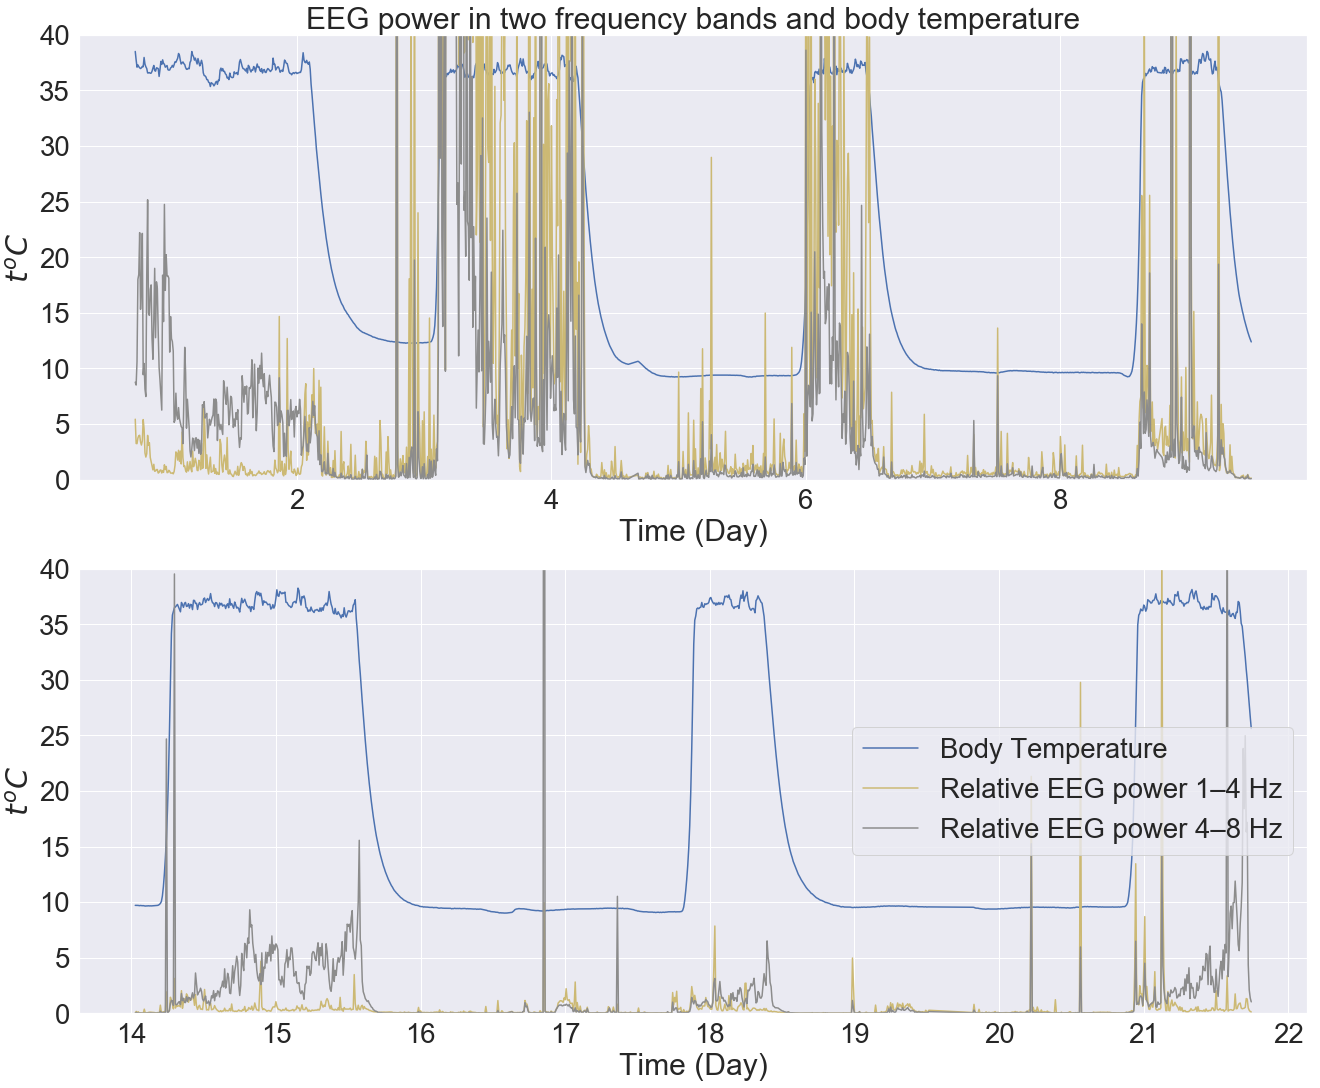
\includegraphics[width=0.7\linewidth]{exp1_3.png}
\caption{The graph shows the hamster body temperature versus time and scaled EEG power values ​​in two different frequency bands (1-4 Hz and 4-8 Hz). The part with a large artifact, located in the middle of the record, is deleted. The graph is divided into two parts for convenience.}\label{fig:lactate_receptors}
\end{figure}
\end{frame}

\begin{frame}[fragile]{The First Hamster}
\begin{figure}[H]
\centering
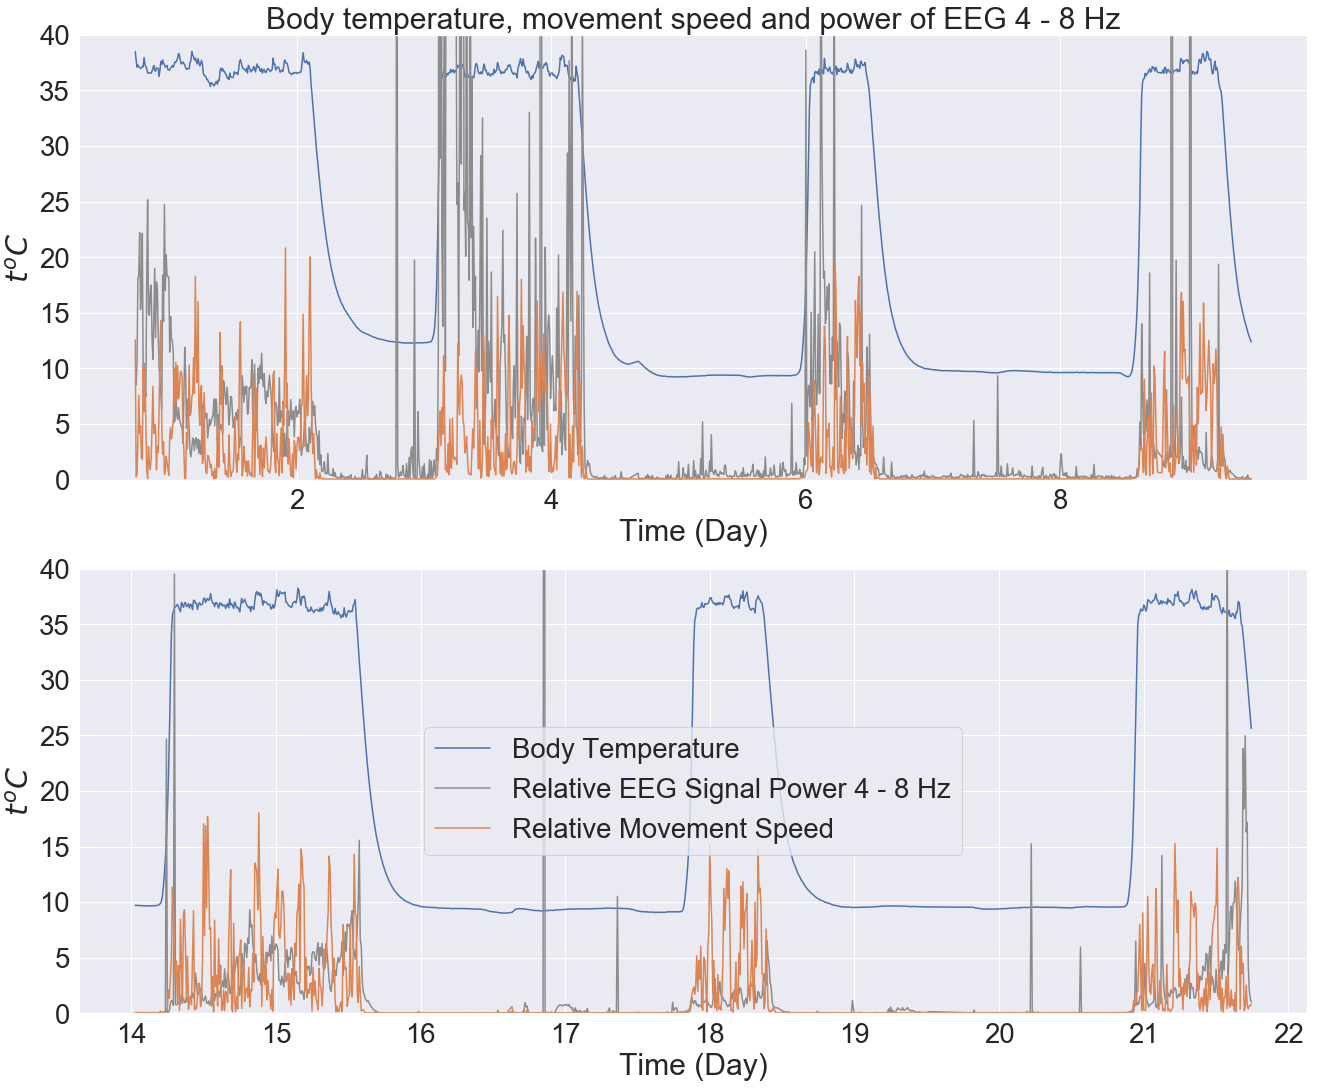
\includegraphics[width=0.7\linewidth]{exp1_4.png}
\caption{The graph shows the body temperature of a hamster as a function of time, scaled movement speed and scaled values ​​of the EEG power in the frequency range 4--8 Hz. The part with a large artifact, located in the middle of the record, is deleted. The graph is divided into two parts for convenience.}\label{fig:lactate_receptors}
\end{figure}
\end{frame}

\begin{frame}[fragile]{The First Hamster}
\begin{figure}[H]
\centering
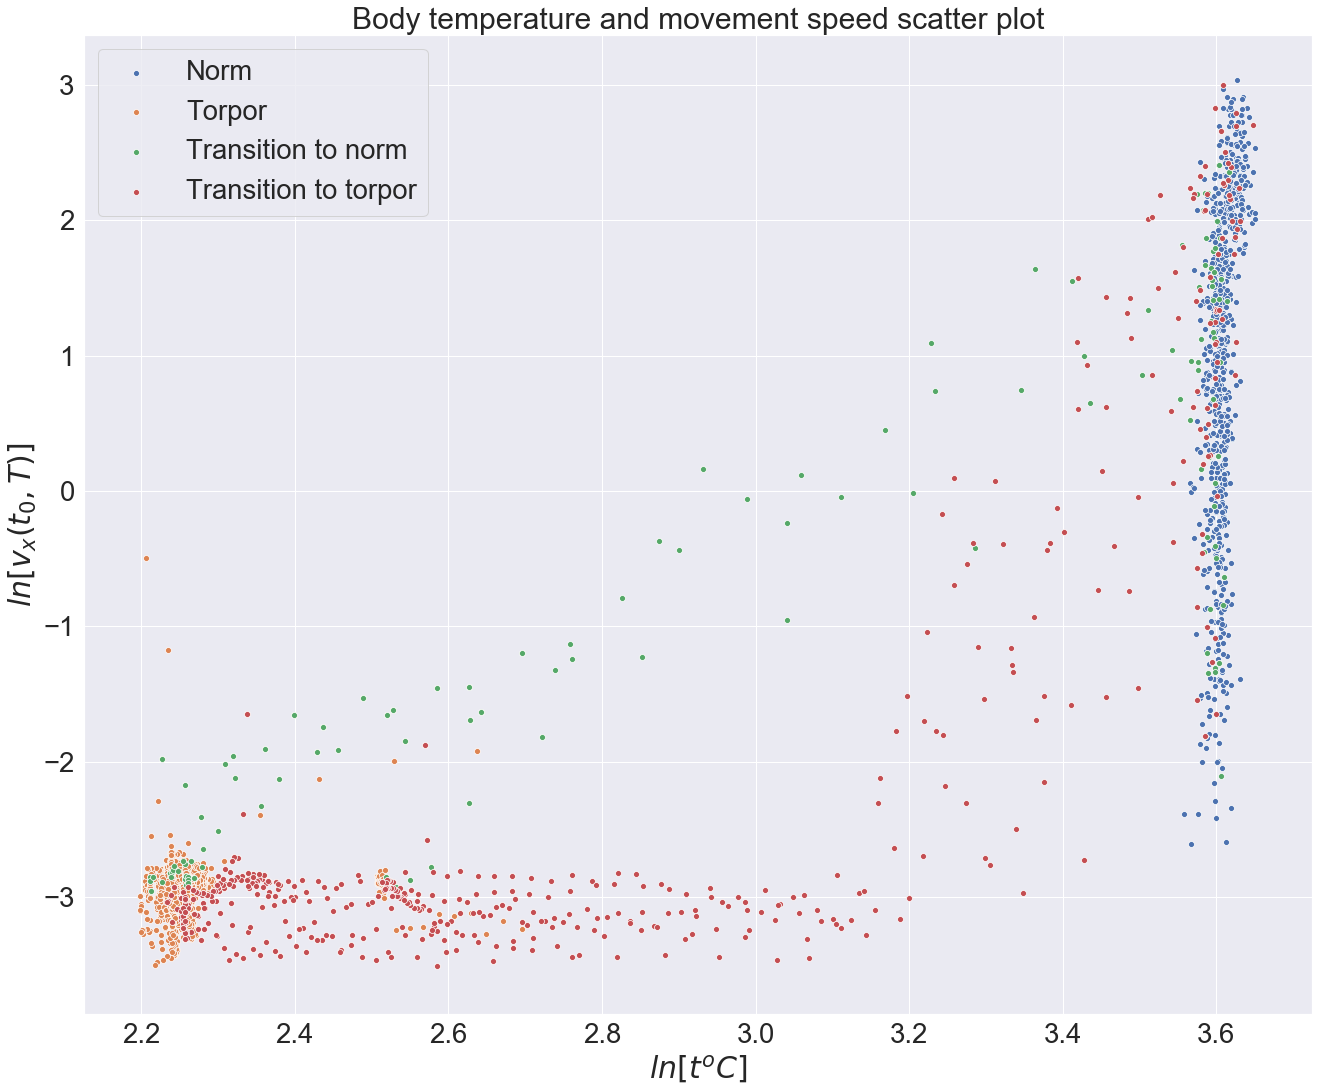
\includegraphics[width=0.7\linewidth]{exp1_5.png}
\caption{The graph shows the scatterplot of the logarithm of the velocity of movement and the logarithm of body temperature, allowing to distinguish four states: norm, torpor, transition to torpor and transition to norm. States are highlighted in colors.}\label{fig:lactate_receptors}
\end{figure}
\end{frame}


\begin{frame}[fragile]{The First Hamster}
\begin{figure}[H]
\centering
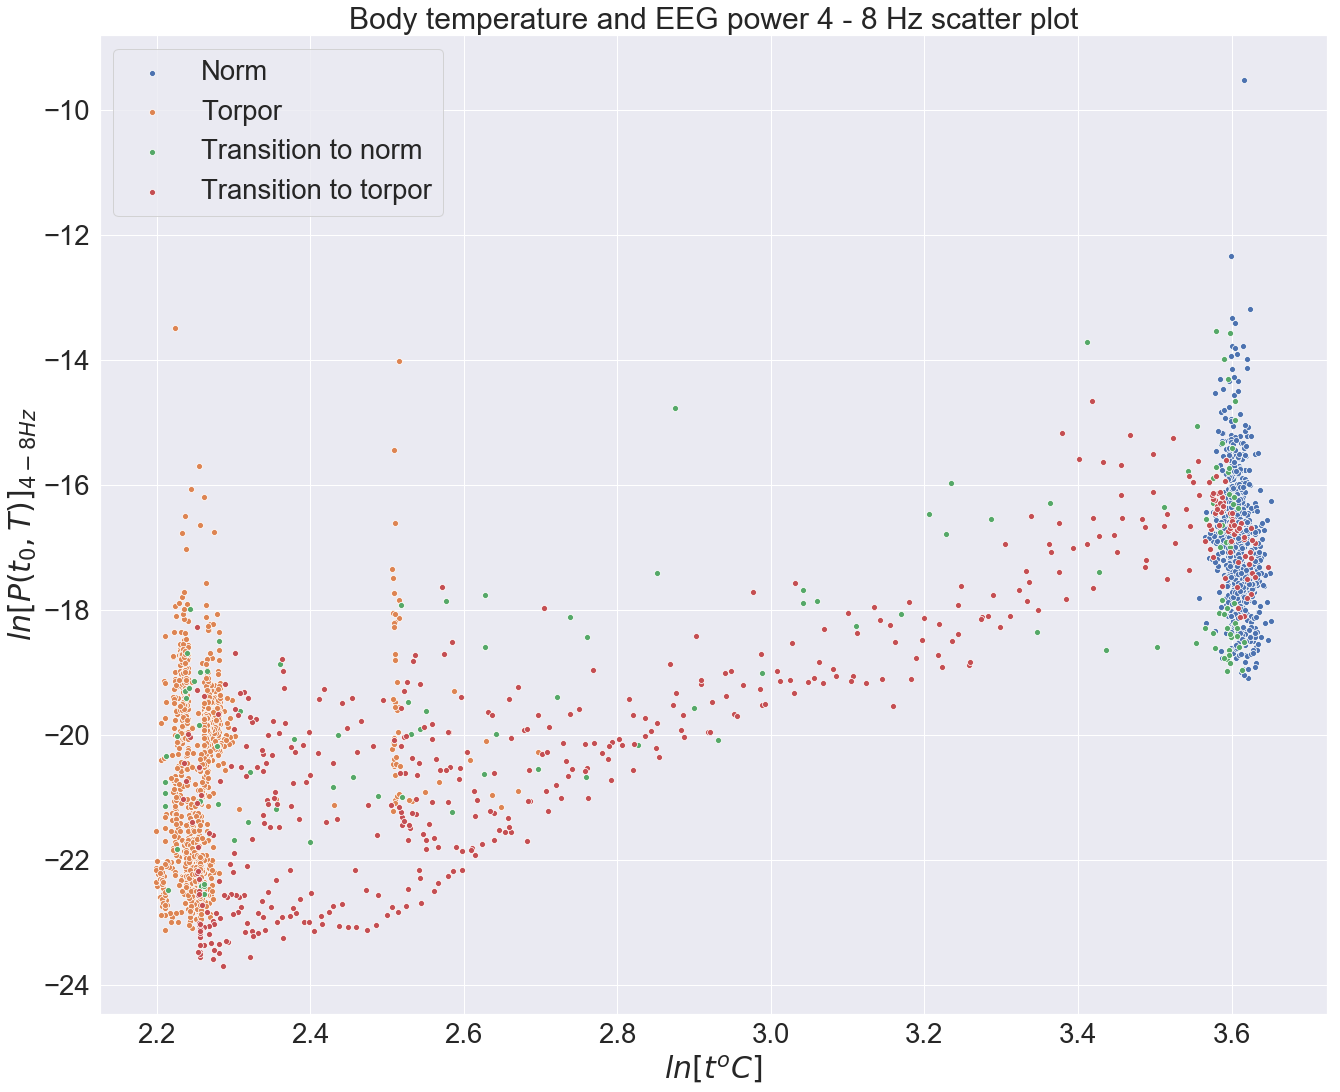
\includegraphics[width=0.7\linewidth]{exp1_6.png}
\caption{The graph shows the scatterplot of the logarithm of body temperature and logarithm of the EEG power in the range of 4-8 Hz. 4 states are selected, corresponding to the diagram of the logarithm of the velocity of movement and the logarithm of temperature.}\label{fig:lactate_receptors}
\end{figure}
\end{frame}

\begin{frame}[fragile]{The First Hamster}
\begin{figure}[H]
\centering
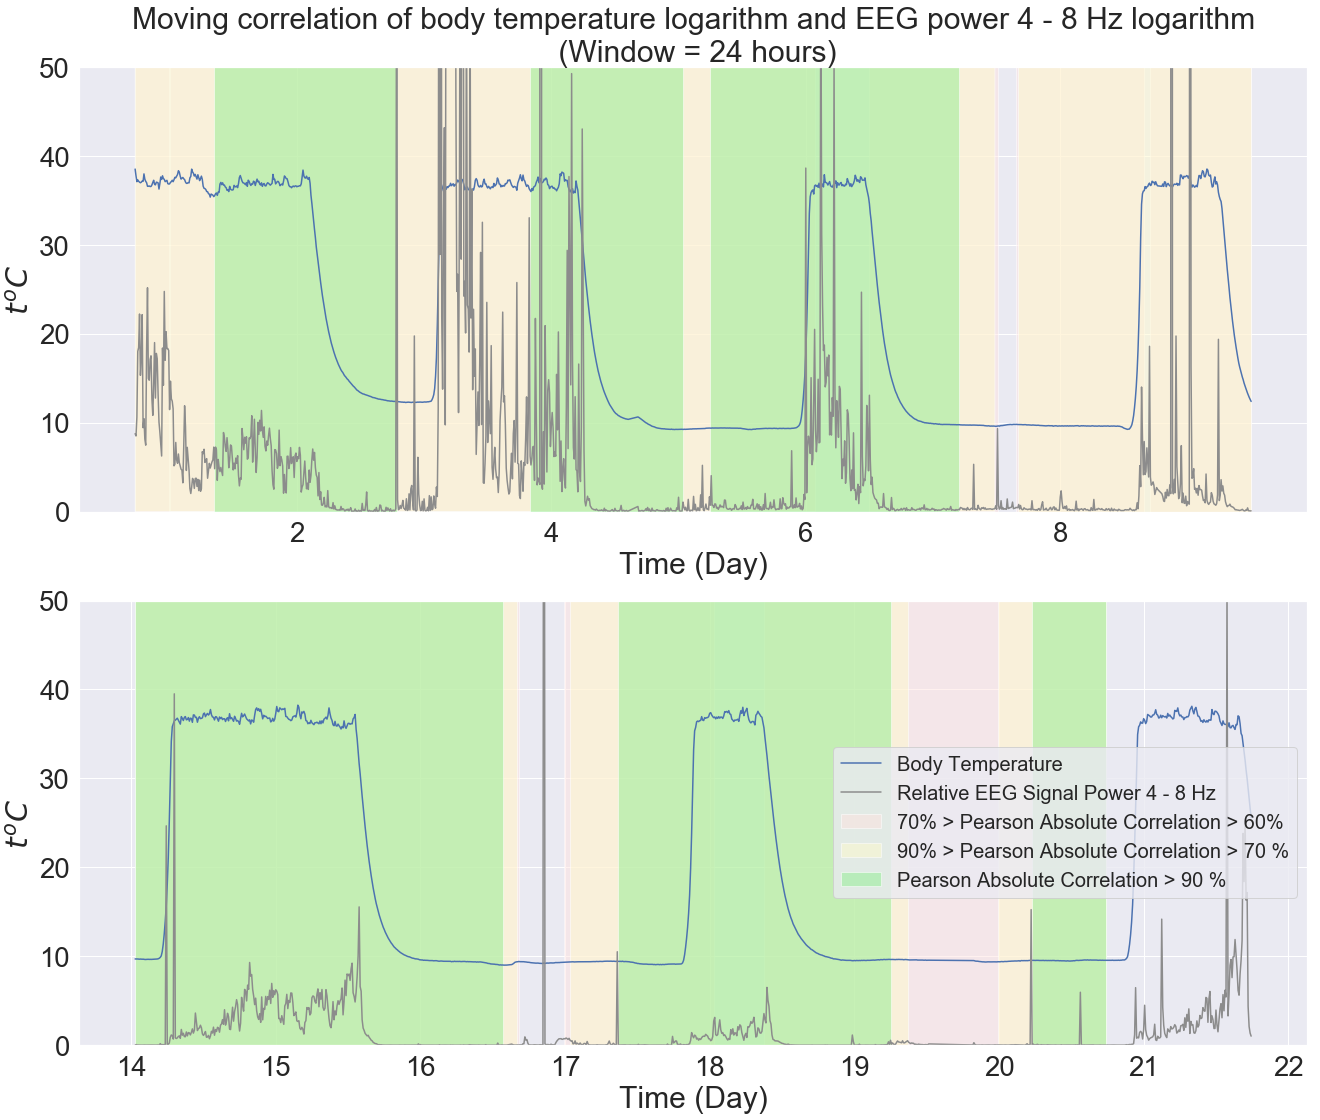
\includegraphics[width=0.6\linewidth]{exp1_7.png}
\caption{The graph shows the body temperature as a function of time; scaled EEG power. Red, yellow and green colors indicate areas where the Pearson correlation between the logarithm of hamster's body temperature and logarithm of EEG power values are significant and have a high value.}\label{fig:lactate_receptors}
\end{figure}
\end{frame}

\begin{frame}[fragile]{The Second Hamster}
\begin{figure}[H]
\centering
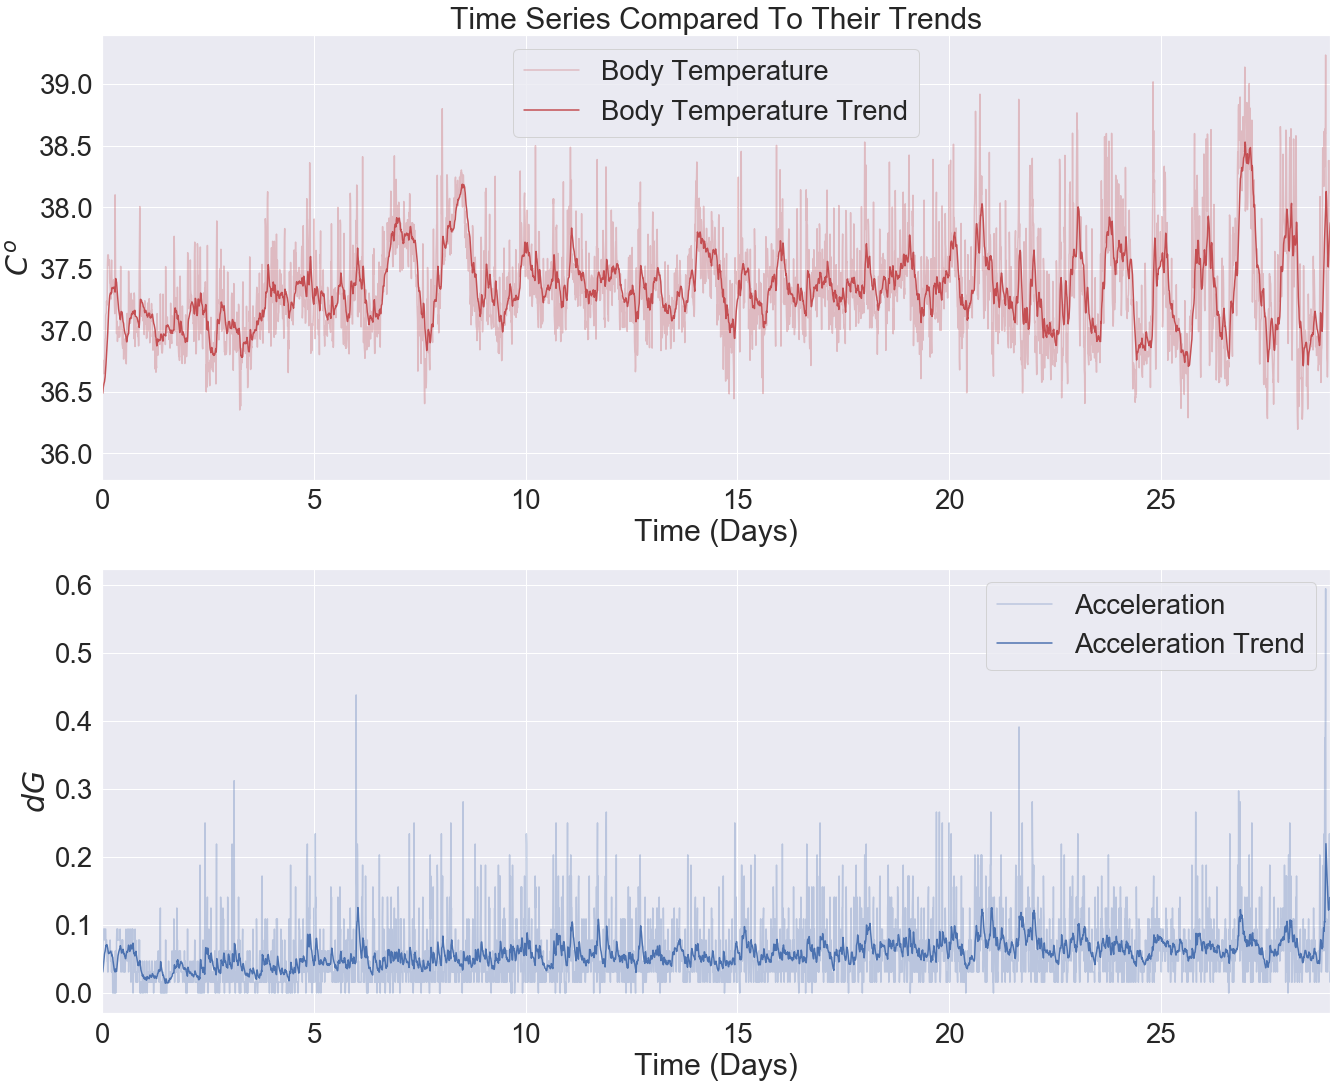
\includegraphics[width=0.6\linewidth]{exp2_1.png}
\caption{Trends of body temperature and acceleration of a hamster against the background of time series.}\label{fig:lactate_receptors}
\end{figure}
\end{frame}

\begin{frame}[fragile]{The Second Hamster}
\begin{figure}[H]
\centering
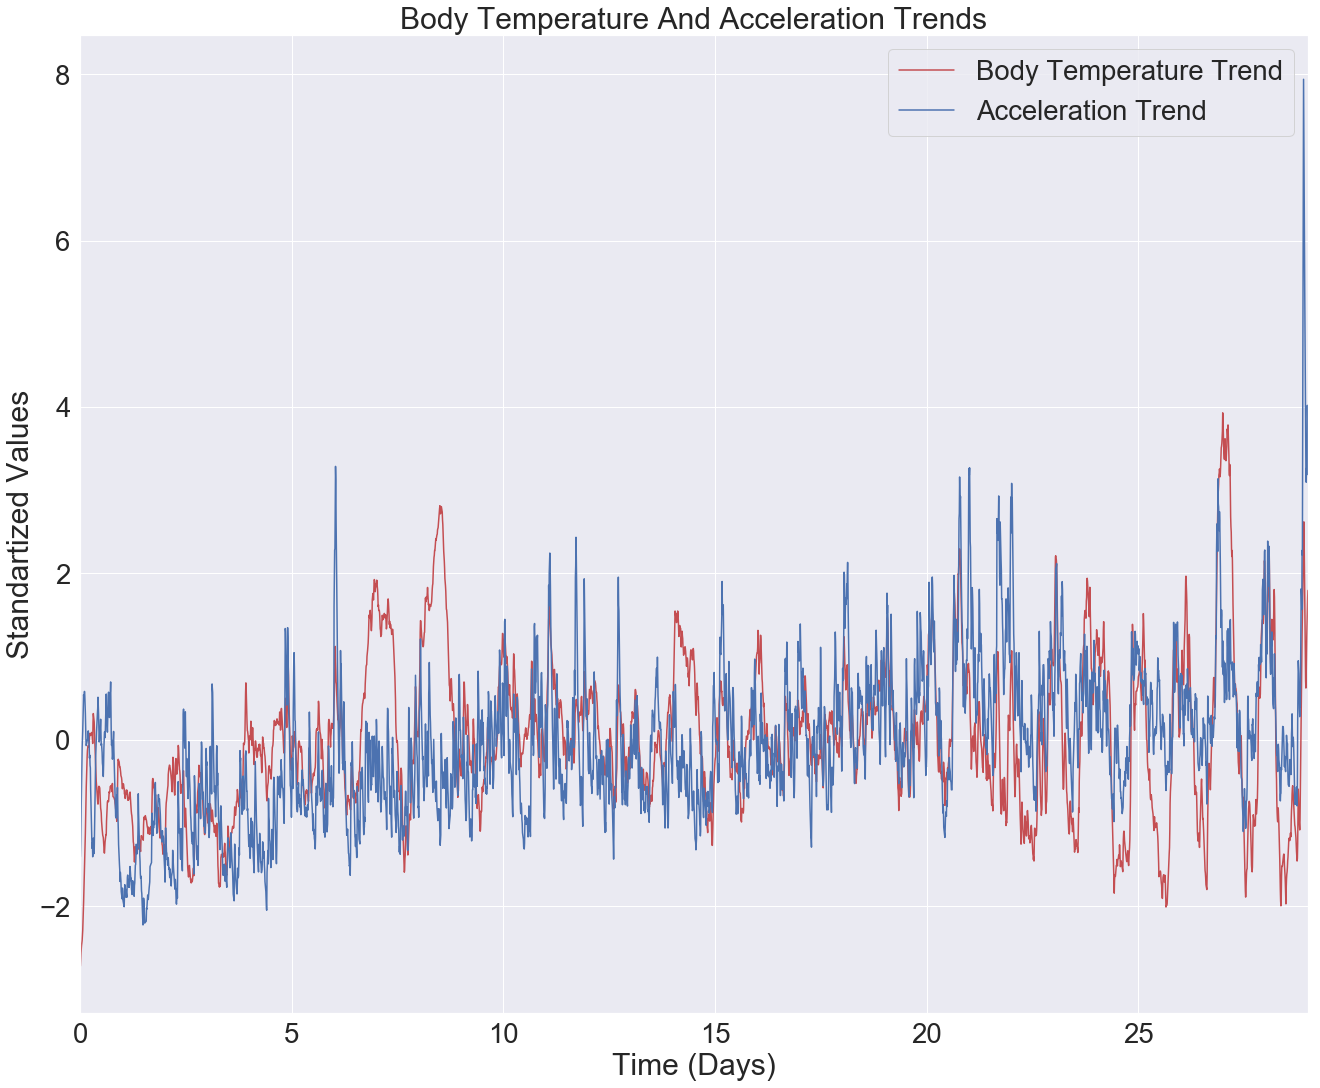
\includegraphics[width=0.6\linewidth]{exp2_2.png}
\caption{Trends of body temperature and hamster acceleration superimposed.}\label{fig:lactate_receptors}
\end{figure}
\end{frame}

\begin{frame}[fragile]{The Second Hamster}
\begin{figure}[H]
\centering
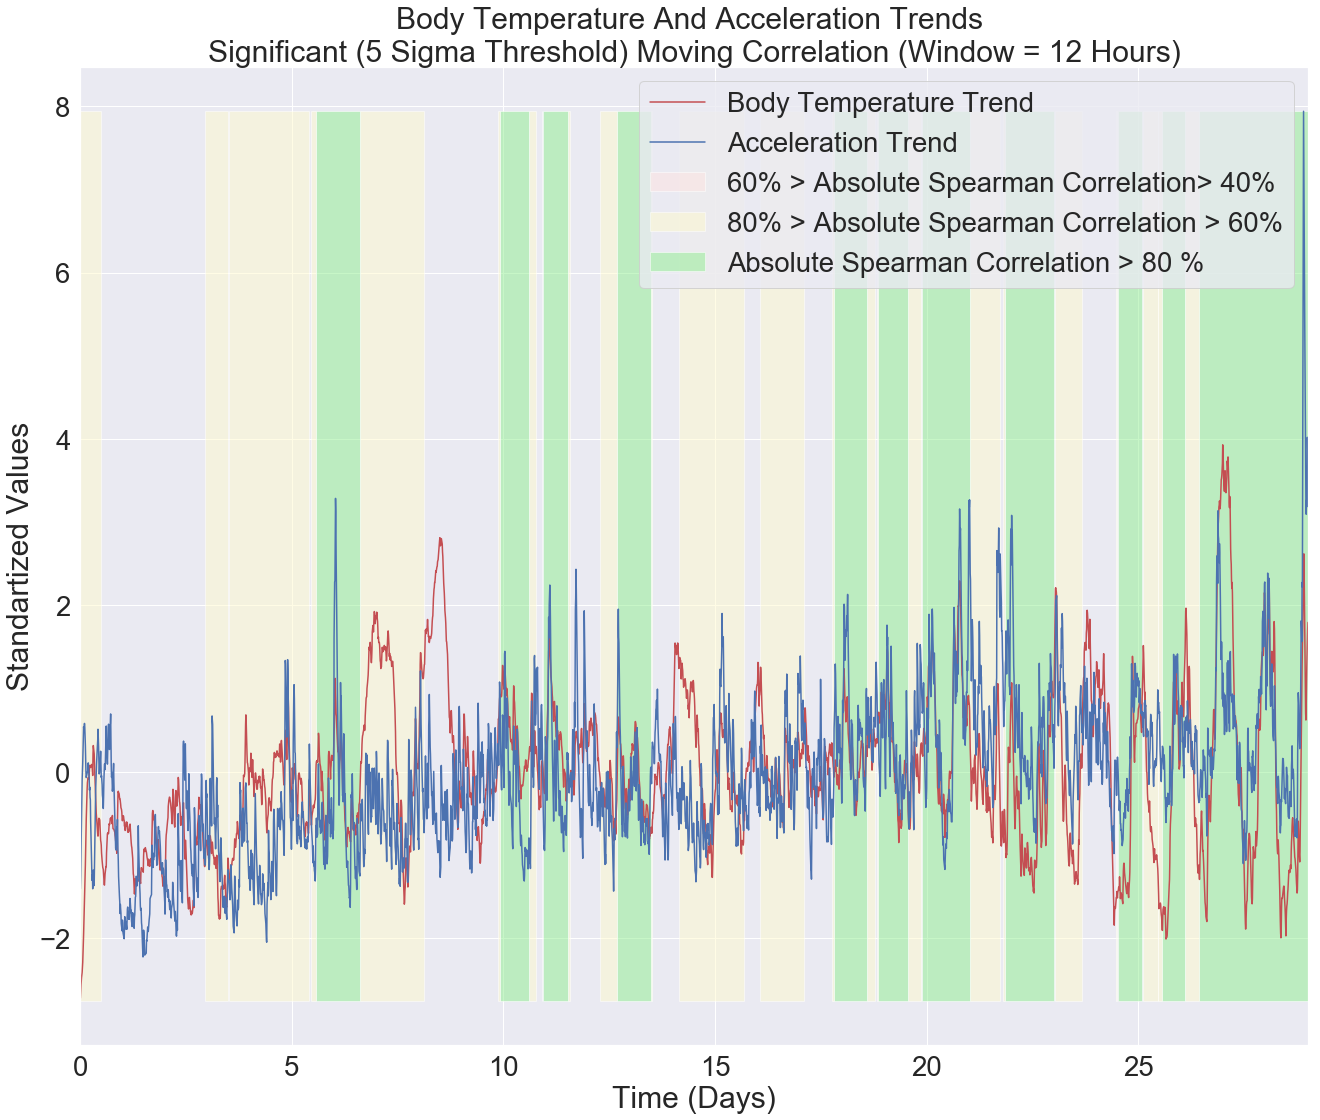
\includegraphics[width=0.6\linewidth]{exp2_3.png}
\caption{The graph shows the body temperature of the hamster as a function of time and scaled values of the speed. Red, yellow and green colors indicate areas where the Sperman correlation between the hamster's body temperature and speed values are significant and have a high value.}\label{fig:lactate_receptors}
\end{figure}
\end{frame}

\section{The Naked Mole-Rat Experiment}

\begin{frame}[fragile]{Naked Mole-Rat}
\begin{figure}[H]
\centering
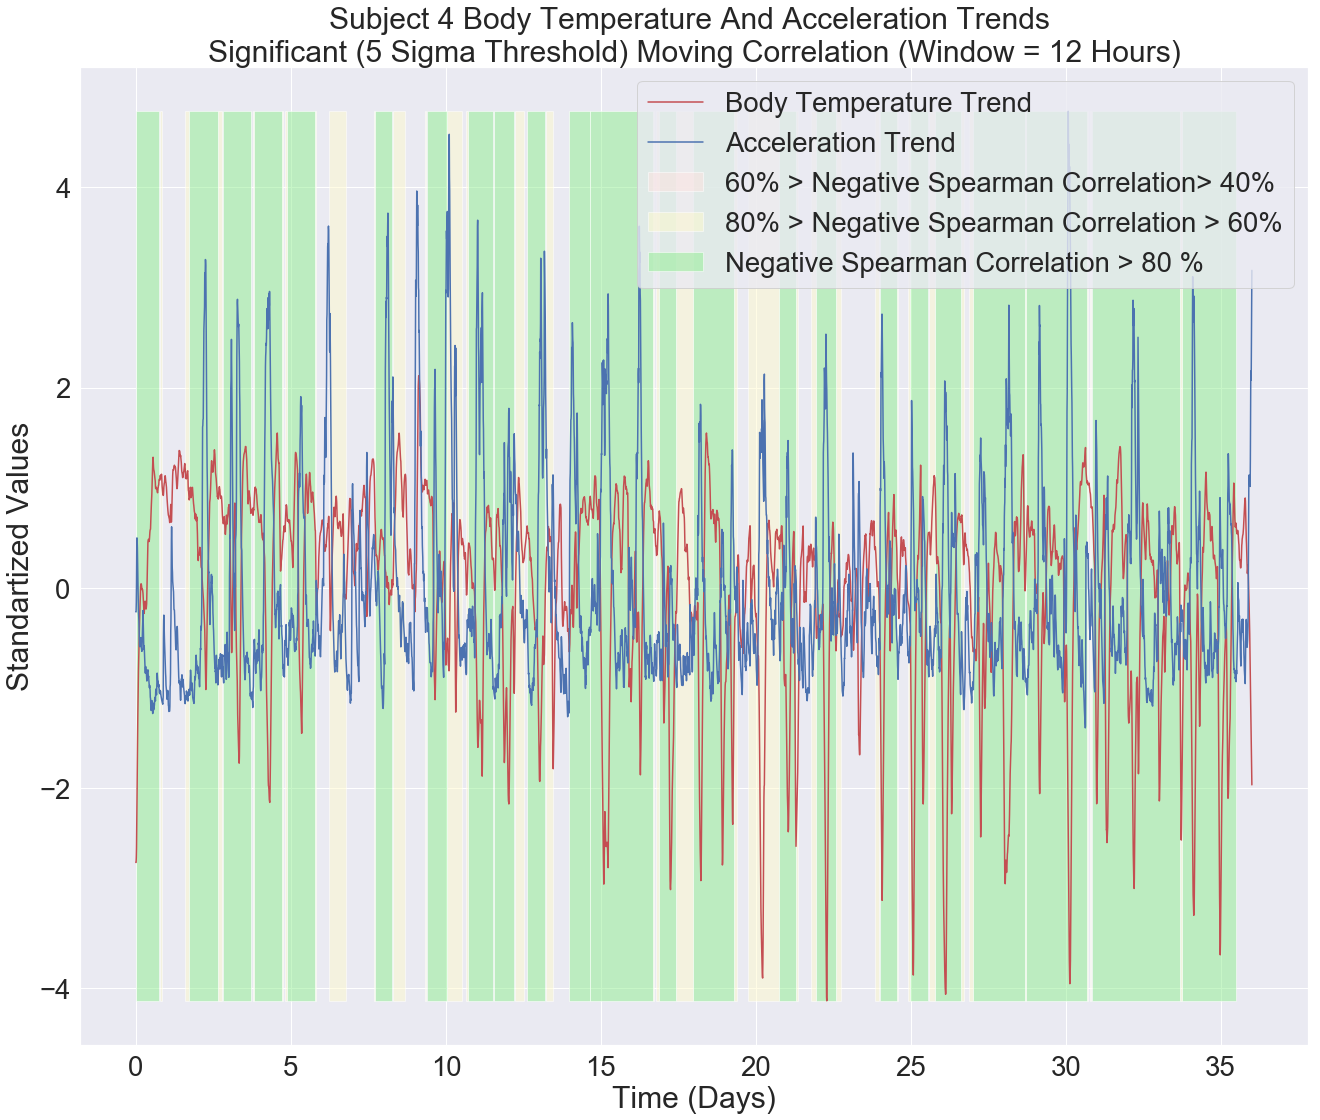
\includegraphics[width=0.6\linewidth]{exp3_4.png}
\caption{The picture shows a moving negative correlation of average acceleration and body temperature of a naked mole-rat at 10 minute time intervals. The y axis is the standardized trends values of time series. Different colors of the background indicate a sliding correlation, highlighting the parts of the graph in the case of a larger effect for this window.}\label{fig:lactate_receptors}
\end{figure}
\end{frame}

\section{The Lactate Experiment}

\begin{frame}[fragile]{L-lactate}
\begin{figure}[H]
\centering
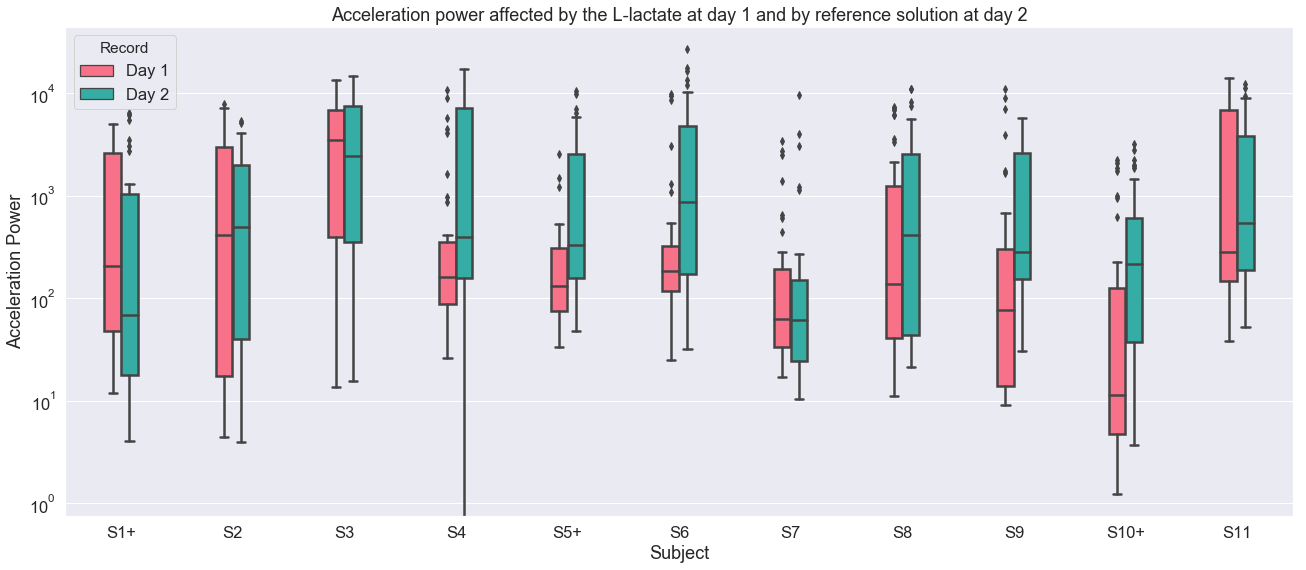
\includegraphics[width=0.9\linewidth]{exp4_1.png}
\caption{The y-axis represents the distribution of the acceleration powers over 10 minute time intervals. On the first day l-lactate was administered to the animal. On the second day reference solution was administered to the animal. A plus in the animal code name denotes a significant difference between distributions on the first and second day.}\label{fig:lactate_receptors}
\end{figure}
\end{frame}

\begin{frame}[fragile]{D-lactate}
\begin{figure}[H]
\centering
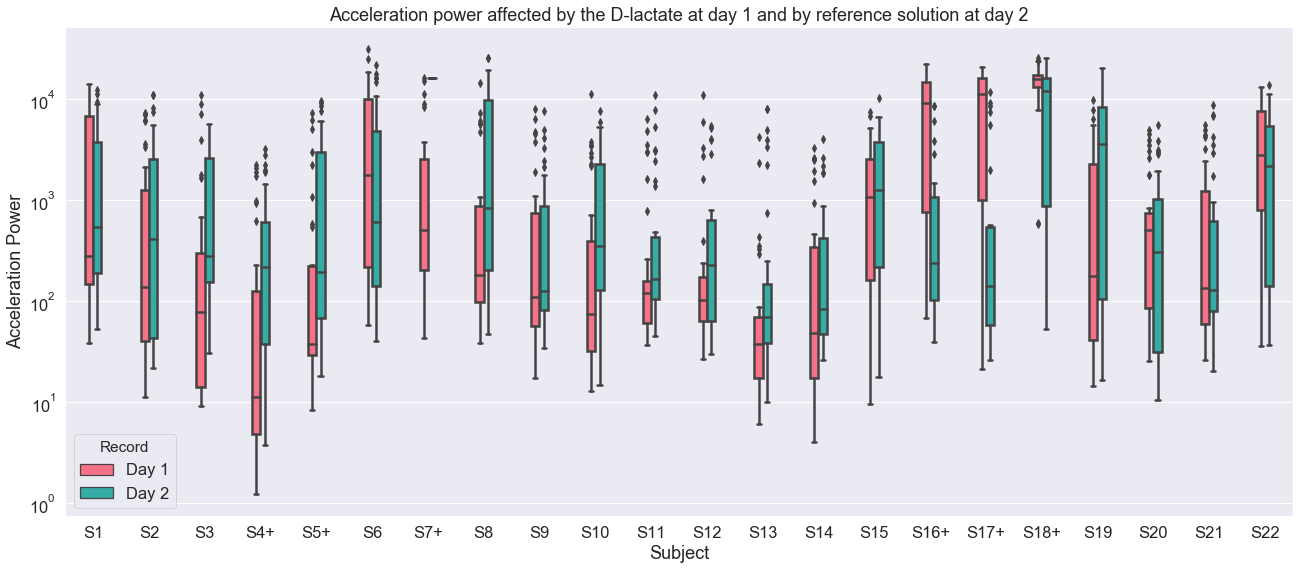
\includegraphics[width=0.9\linewidth]{exp4_2.png}
\caption{The y-axis represents the distribution of the acceleration powers over 10 minute time intervals. On the first day d-lactate was administered to the animal. On the second day reference solution was administered to the animal. A plus in the animal code name denotes a significant difference between distributions on the first and second day.}\label{fig:lactate_receptors}
\end{figure}
\end{frame}

\section{Lactate Receptors Phylogenetic Tree}

\begin{frame}[fragile]{L-lactate receptors}
\begin{figure}[H]
\centering
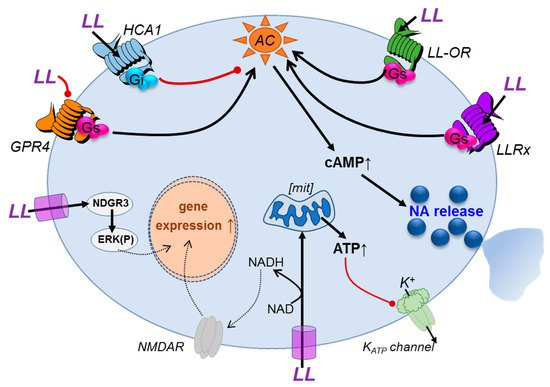
\includegraphics[width=0.7\linewidth]{lactate_receptors.jpg}
\caption{"AC — adenylate cyclase; ERK(P) — phosphorylation of extracellular signal–regulated kinases; GPR4 — orphan G-protein-coupled receptor 4; HCA1—hydroxy-carboxylic acid receptor; LL-OR — LL-activated olfactory receptor; LLRx — LL receptor on noradrenergic neurones; [mit] — mitochondria; NA — noradrenaline; NMDAR — NMDA receptor." \citep{Mosienko2018}}\label{fig:lactate_receptors}
\end{figure}
\end{frame}

\begin{frame}[fragile]{Phylogenetic Tree}
\begin{figure}[H]
\centering
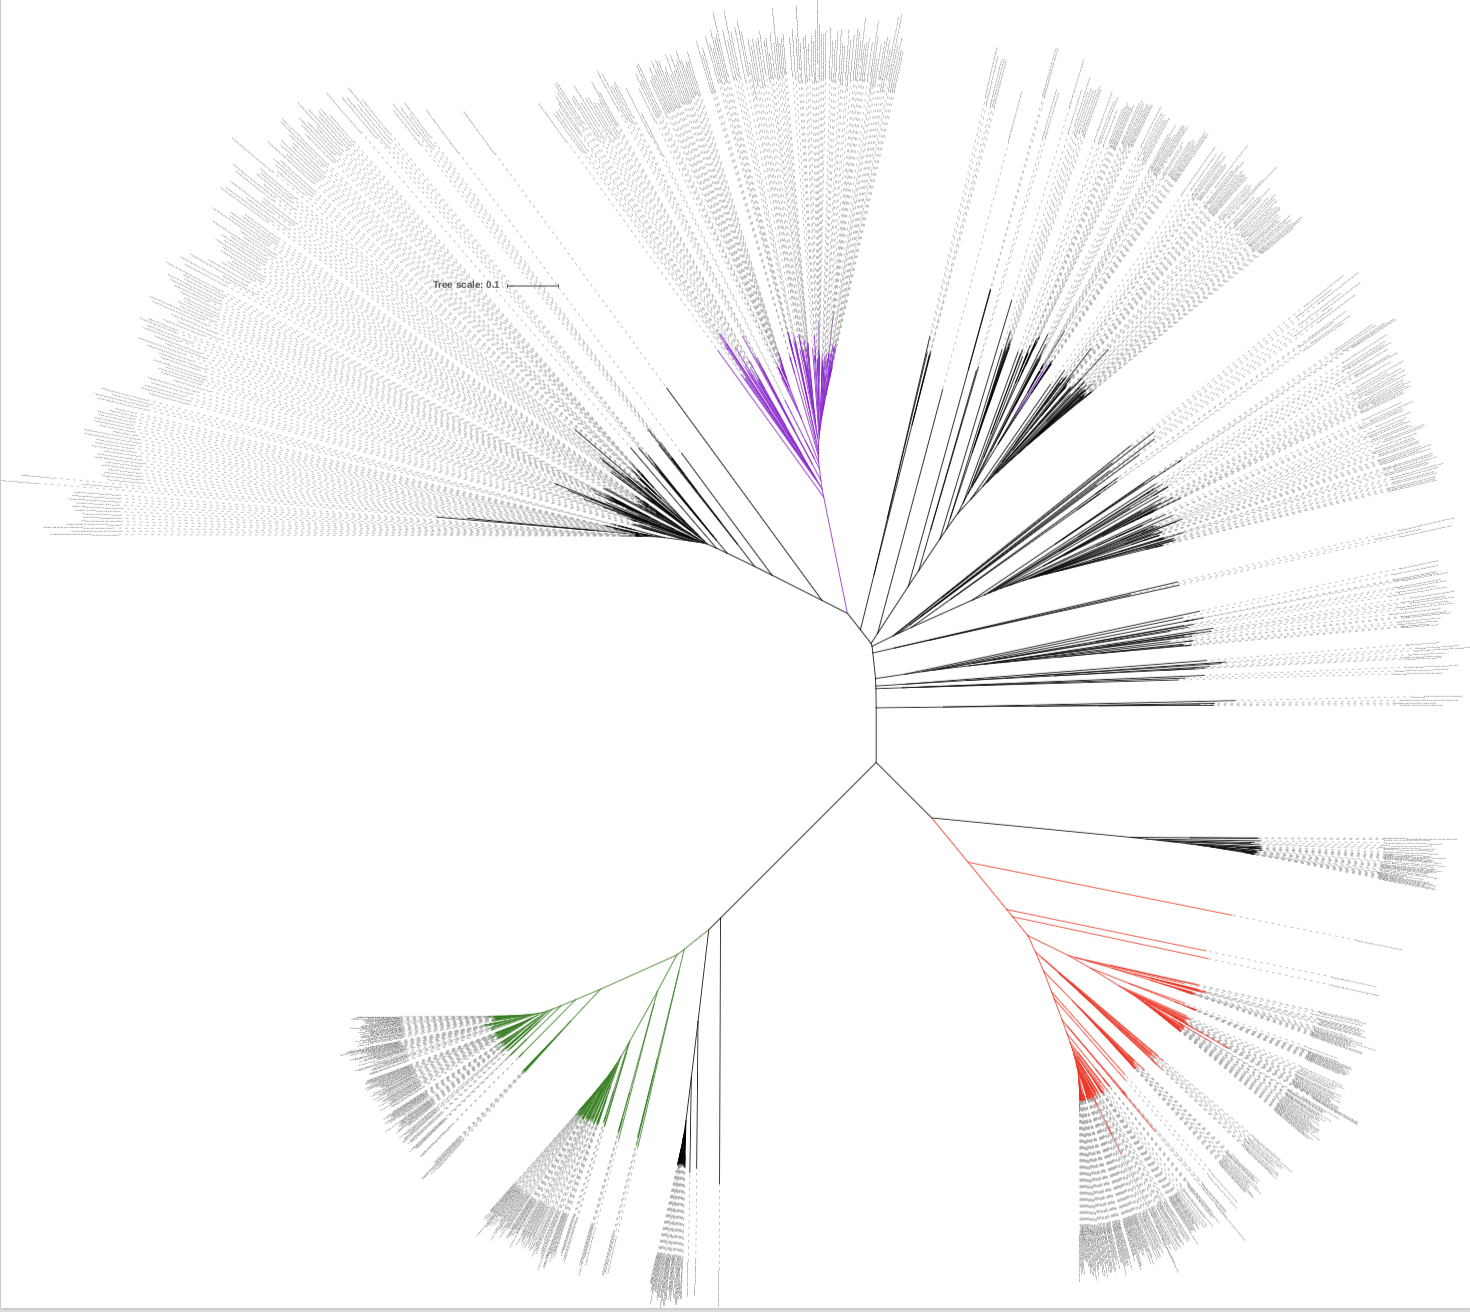
\includegraphics[width=0.7\linewidth]{tree.png}
\caption{GPR – red; HCA1 - purple; LL-OR – green}\label{fig:lactate_receptors}
\end{figure}
\end{frame}

\begin{frame}[allowframebreaks]{References}

\bibliographystyle{apa}
\bibliography{/Users/wassilyminkow/Scripts/LaTeX/library.bib}

\end{frame}

\end{document}
